\chapter{The State of the Art}
In this chapter we will analyze the most recent advances and promising ideas about distributed evolutionary algorithms and web technologies.

\section{Distributed Evolutionary Algorithms}
A distributed Evolutionary Algorithm divides across a set of available processors the different genetic operators involved in a classic EA. In \cite{soa-dea}, Gong et al. made a comprehensive analysis of the sate-of-the-art distributed algorithms that we will use to explain and show the most recent advances on the different distributed models that has gain attraction of researchers in the recent years.

Since most of practical optimization problems show complex interdependence over the different variables involved, we will focus on population-based distributed models which distribute individuals of a population to multiple processors. Rather than pure dimension-distributed models that divide high dimensional complex problems into several lower dimensional and simpler problems.

\begin{table}[h!]
\centering
\addtolength{\leftskip} {-2cm} % increase (absolute) value if needed
\addtolength{\rightskip}{-2cm}
\resizebox{1.3\textwidth}{!}{%
\begin{tabular}{|l|l|l|l|l|l|}
\hline
\multicolumn{1}{|c|}{\textbf{Model}} & \multicolumn{1}{c|}{\textbf{Parallelism level}} & \multicolumn{1}{c|}{\textbf{Search behaviour}} & \multicolumn{1}{c|}{\textbf{Communication cost}} & \multicolumn{1}{c|}{\textbf{Scalability}} & \multicolumn{1}{c|}{\textbf{Fault-tolerance}} \\ \hline
Master-Slave                         & Operation, evaluation                           & Similar to sequential EA                       & Medium $\sim$High                                & Medium                                    & Medium                                        \\ \hline
Island                               & Population                                      & Better Diversity                               & Low $\sim$Medium                                 & Low                                       & Medium $\sim$High                             \\ \hline
Cellullar                            & Individual                                      & Better Diversity                               & Medium                                           & Medium $\sim$High                         & Medium $\sim$High                             \\ \hline
Pool                                 & Population, Individual, Operation               & Depends on design                              & Low                                              & High                                      & Medium                                        \\ \hline
\end{tabular}%
}
\caption{Comparison of population-based distributed models from \cite{soa-dea}. Modified to acknowledge \textit{single point of failure} issues.}
\label{tab:deas}
\end{table}

\subsection{Master-Slave}

It is a centralized model where one node has the role of master and the rest of slaves.
The master owns the entire population and is in charge of applying the genetic operators of selection, crossover, mutation, and replacement. The slaves, on the other hand, do not know about other slaves and are in charge of evaluating the fitness of the chromosomes in the population of the master.

The fitness function must require the majority of the computing load, otherwise, a non-distributed approach will outperform this model since the communication between the master and its slaves will be a bottleneck. 

In order to to apply this model to problems where the fitness function computational cost is not high enough, recent researches suggest to distribute other operators such as the crossover or mutation \cite{ismail}, or applying local search on slaves \cite{zhang2}. 

Another way to deal with this kind of problems is having a subpopulation in each slave; it will apply all the genetic operators and will communicate the best chromosomes within its population to the master. The master will be in charge of sending the best chromosomes to all its slaves.\cite{zhang1}

Although this model is simple and therefore easy to prototype, it has important limitations. The master's performance and communication time limits the performance scalability of this model \cite{erick}. Also, even though this model is fault tolerant across slaves (a failing slave can be replaced by a working one), the master still represents a single point of failure in this approach.

\subsection{Island}

Traditional evolutionary algorithms suffer from premature convergence problems when all chromosomes are around the same local optima. In this model, global search is improved with a rather simple design.

A population is divided into as many subpopulations as processors. Chromosomes migrate from one island to another at a set interval, this is equivalent to the selection operator in the source island and replacement in the destination one.

All islands should end up having the best solution so far within their subpopulations. This can be achieved either synchronously after an specific number of generations \cite{89}, or asynchronously when it is ready \cite{30}. Whereas the synchronous approach is simpler, the asynchronous approach is more flexible and can achieve better efficiency.

An important design decision for a island distributed EA is the topology of the islands. Whitley et al \cite{140} conducted an experiment where all islands were fully connected without using any kind of topology. They found that if the migration is conducted among all islands, the algorithm achieves almost the same results as a sequential execution. In recent years, different network topologies for island models have been being studies. Network topologies such as ring, torus, or layered have achieved superior performance in different experiments. \cite{62}

Scalability of this model is limited since performance highly depends on the number of islands and its resulting granularity \cite{58}. However, it has a good partition-tolerance since, although a failing island means a lost important portion of the entire population, it does not have any single-point of failure.

\subsection{Cellular}
In this model the entire population is distributed across all processors. Ideally one chromosome per processor. Communication between processors is defined by a network topology where chromosomes can only compete and mate with its neighbors.

If this model follows a synchronous approach, all cells update their chromosome simultaneously. Otherwise, cells update their chromosomes one by one asynchronously.

Alba et al. \cite{2} compared asynchronous and synchronous cellular-based models, solving discrete and continuous problems. They found that for discrete problems, asynchronous are more efficient, whereas synchronous find solutions with better fitness. For continuous problems, the opposite happened.

The topology plays an essential role in this mode as well. In \cite{68}, experimental results shown that for simple problems a regular topology (with high mean degree distribution) achieves better results. On the other hand, for complex problems a more complex network with high clustering coefficient is preferred.

Also, the ratio between the neighborhood radius and the topology radius plays a similar role as the topology itself. For simple problems a higher ratio achieves better results, whereas for complex problems a low ratio is preferred.\cite{5}

Cellular models are suitable to be easily implemented as a decentralized system. When dealing with a decentralized population where processors (alongside chromosomes) can join and leave without notice, it is very important to maintain the population size within bounds in order to avoid the population to explode or implode. 

Wickramasinghe et al. \cite{p2p-ea} developed a peer-to-peer cellular EA with adaptive selection that decided whether a chromosome is good enough to mate with a neighbor or not with the following probabilistic function:

\begin{equation}
    P(x) = sig_{m,s}(\Delta f(x)) = \frac{1}{1 + e^{-m \cdot (\Delta f(x)-s)}}
\end{equation}

Where $s$ and $m$ are adjustable variables that respectively determines where the transition from low probabilities to high probabilities takes place and how sharp that transition is. These variables are automatically adjusted by the algorithm.

As previously stated, topology is a key issue and even more in a peer-to-peer network. J.J Merelo et al \cite{evag} achieved promising results using the \textit{Newscast} protocol, a dynamic and self-organized gossiping protocol for the maintenance of unstructured P2P overlay networks \cite{newscast}, as topology builder and neighborhood policy.


\subsection{Hierarchical}
Also known as Hybrid models, they combine different distributed models in order to take advantage of the problem-solving and scalability capabilities of the models they are made of.

\paragraph*{Island \& Master-Slave.} The population is split into several subpopulations across different master nodes. At the same time, these subpopulations will be islands where periodically chromosomes will migrate from one master node to another. A master sends chromosomes from its island to its own slaves, which will evaluate the chromosome fitness function.

This model addresses the scalability shortcoming of the island-based model as well as avoids the single point of failure that the unique master server represented. Moreover, the speedup of this hybrid model is relatively linear \cite{13}.

\paragraph*{Island \& cellular} Multiple processors that store a cells each one, are combined into groups of cells that will behave as islands. The quality of the solutions this model finds are comparable to classical distributed models but it provides better scalability and fault-tolerance.

\paragraph*{Island \& Island} When processors in island-model model are heterogeneous, but the model itself is homogeneous (all islands share the same settings of operators, control parameters, fitness evaluations, etc...), slower processors will slow-down the entire algorithm execution. Furthermore, a homogeneous model may not keep a proper balance between exploitation and exploration.  

Heterogeneus island models are being developed in order to address that issue. Sefrioui et al \cite{112}. designed a layered island model of three layers where the first layer was in charge of exploiting the already explored solution space, the second layer balanced exploitation and exploration, and the third one was fully-exploratory.

According to Herrera et al \cite{57}, local and global migration methods are a key issue in these hierarchical models since these methods establish the actual hierarchy between the layers. This approach achieved promising results in Herrera's hierarchical design approach, improving efficiency and collaboration. 

\subsection{Pool}
A pool storing chromosomes is shared between processors that do no know each others. The pool is divided into as many segments as processors. A processors can take any chromosome within the entire population, but can only overwrite a chromosome in its assigned segment to avoid race conditions.

Processors randomly reads as many chomosomes from the pool as they have within their segments. Then, after applying genetics operators, they replace the chromosomes on their segment with the resulting offsprings that have better fitness than the original. 

Since processors do not know each other and race conditions are under control, asynchronization and heterogeneity are almost intrinsic properties on this model. Moreover, new processors can easily join and leave asynchronously by dynamically resizing the segments each processor has.

As in Marter-Slave, the pool in this model is a single point of failure that limits the fault tolerance of the system. Replication of the pool can help to address this issue by backing up the state of the pool in case it goes down during the execution of the algorithm. 

\section{Web Technologies}
Dynamic websites are capable of showing different information based on the context and actions made by a user. The logic behind the shown information can be handled by either the server that serves the website or the user's web browser. 

\subsection{Server-Side processing}

In server-side scripting, the webpage that will be served to the user as a response to a request with given set of parameters, is completely build by the server that handles the request. Therefore all the computation to reason and compose the entire new webpage is handled by the server while the client browser only shows the resulting information without reasoning about it.

The logic behind the server, also known as \textit{backend}, can be implemented in almost any language although specialized frameworks and stacks are being developed in popular languages such as:

\begin{enumerate}[a)]
	\item \textbf{PHP.} The LAMP stack \cite{lamp} which stands for \textit{Linux, Apache, MySQL, PHP} is a widely adopted architecture where requests are handled by the Apache HTTP server and processed by PHP scripts that retrieve information from a relational database.

	\item \textbf{Python.} Django \cite{django} which follows a Model-View-Controller (MVC) architecture. It comes with out of the box support for user authentication, security analysis, database integration, and administration GUI. Examples of major sites using this framework are \textit{Instagram}, \textit{Bitbucket}, or \textit{Pinterest}. \cite{django-websites}
	
	\item \textbf{Ruby.} Rails adopts the MVC architecture as well. It comes with the benefits of ruby like rapid-development and easy deployment and configuration. Major websites using this framework are \textit{GitHub}, \textit{Airbnb}, or \textit{Shopify}. \cite{rails}
\end{enumerate}

\subsection{Client-Side processing}
In order to relieve the server from building the entire webpage, client-side scripting is used to handle actions made by the user in the browser itself. JavaScript is the most widely adopted scripting language used to develop dynamic webpages \cite{js_stats}, and major web browsers comes with dedicated JavaScript engines built in.  

JavaScript scripts are embedded in or included from HTML and interact with the webpage by manipulating its DOM; a tree-like structure where each node is an object that represents a part of the webpage. 

In 2008, Google released \textit{Chrome V8} \cite{chrome_v8}, the open-source JavaScript engine that powers \textit{Google Chrome}. Contrary to other engines which just intepret JavaScript, V8 compiles JavaScript to native machine code before executing it as well as dynamically optimizes it at runtime.

Firefox, on the other hand, uses SpiderMonkey which compiles to native code critical parts of the scripts to be executed \cite{tampermoneky}. The remaining code that is not compiled to native code is compiled to a special byte-code which although is not as fast as native code, it is faster to compile.

A comparison between these two browsers can be obtained in \cite{firefox_benchmark}. As we can see, in the most recent releases of both browsers, Chrome V8 has the best overall performance.

\subsection{Hybrid approach}
Speak about using both client side scripting and server side scripting and comunication methods such as (g)RPC, HTTP Rest, etc...

Webpages often take a hybrid approach where the DOM is manipulated client-side but certain information is obtained server-side since there are specific tasks that should not or cannot be performed in the client because they can require access delicate information or high processing power. This information is usually requested to a server by using a SOAP, REST or gRPC service.

\begin{enumerate}[a)]
	\item \textbf{SOAP.} \textit{Simple Object Access Protocol} \cite{SOAP} uses XML to transfer structured information over a variety of underlying protocols. SOAP is an official protocol that comes with its own specification so that, although it provides guarantees over reliability and security among other properties for more intricate systems, it has an extra complexity and therefore it requires more bandwidth and resources than other alternatives.

	\item \textbf{REST.} Stands for \textit{Representational State Transfer}. Contrary to SOAP or RPC, it is not a protocol by itself but rather a software architectural style that defines certain design patterns to be followed in order to develop stateless and loosely coupled applications where information is exchanged over HTTP. REST aims to provide easy cacheability and self-descriptive messages where, by using  the different HTTP  methods, a resource identified by a given URI can be created, retrieved, modified or deleted. 
	
	REST applications often use JSON as data representation method since it is more human readable and faster to serialize and deserialize than XML. Also, since REST inherits HTTP methods, requesting information to a server is easier than with SOAP.

	\item \textbf{RPC.} Abbreviation of Remote Procedure Call, it is a remote method invocation protocol where a client can request a server to execute a subroutine and get its result. RPC enables the programmer to invoke that remote procedure as if it was a local procedure, without the programmer explicitly coding the underlying communication.
	
	After using it internally for years, Google released gRPC \cite{grpc} in 2015; an open source RPC system that uses HTTP for transport. Data serialization and interface definition is made with Protocol Buffers; Google's language-neutral, platform-neutral and extensible solution for serializing structured data \cite{protobuf}.
	
	As seen in Figure \ref{fig:protobuff_json_xml}, by using Protocol Buffers, gRPC is able to outperform JSON and XML serialization time and in-memory size. In 2019, gRPC announced support for web-browsers \cite{grpc-web-announce} and positioned as an promising alternative to REST and SOAP. 
	
	\begin{figure}[h!]
		\centering
    	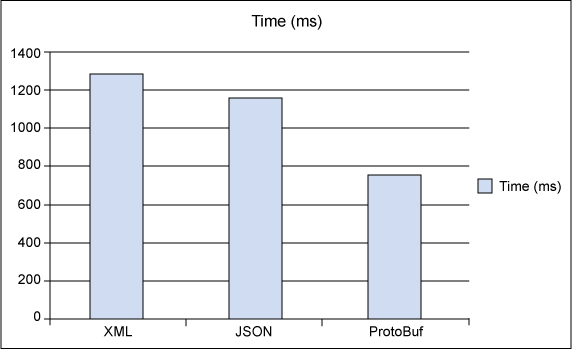
\includegraphics[width=0.45\linewidth]{assets/images/protobuff-json-xml_rw.png}
    	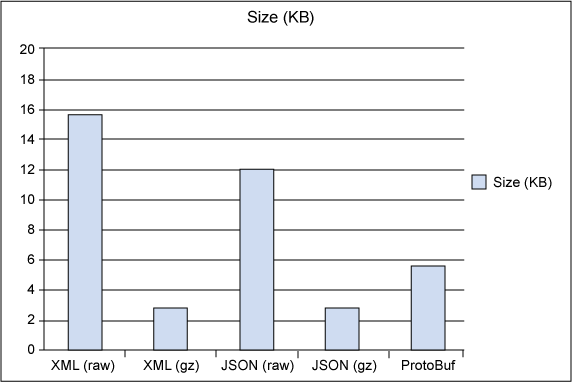
\includegraphics[width=0.45\linewidth]{assets/images/protobuff-json-xml_size.png}
    	\caption{Comparison of serializarion time and serialization in-memory (raw) size of JSON, XML and Protocol Buffers. \cite{protobuff_json_xml}}
    	\label{fig:protobuff_json_xml}
	\end{figure}
	
 \end{enumerate}






\subsection{Web Assembly}
Mention that before wasm you had to either spend a lot of more computation time in the browser with JS or do it faster in the backend. Now you can use wasm to run computation-intense tasks in the client.

Speak about how it works.